\section{Frontend}

L'application en l'état est disponible et jouable à l'adresse suivante \href{https://place.beescreens.ch}{place.beescreens.ch}.

\subsection{Présentation de l'interface}

Voici tout d'abord quelques figures présentant l'interface sur ordinateur ainsi que sur mobile. La différence principale entre les deux versions est le menu permettant à l'utilisateur de choisir la couleur de son pixel.


\begin{figure}[H]
  \centering
  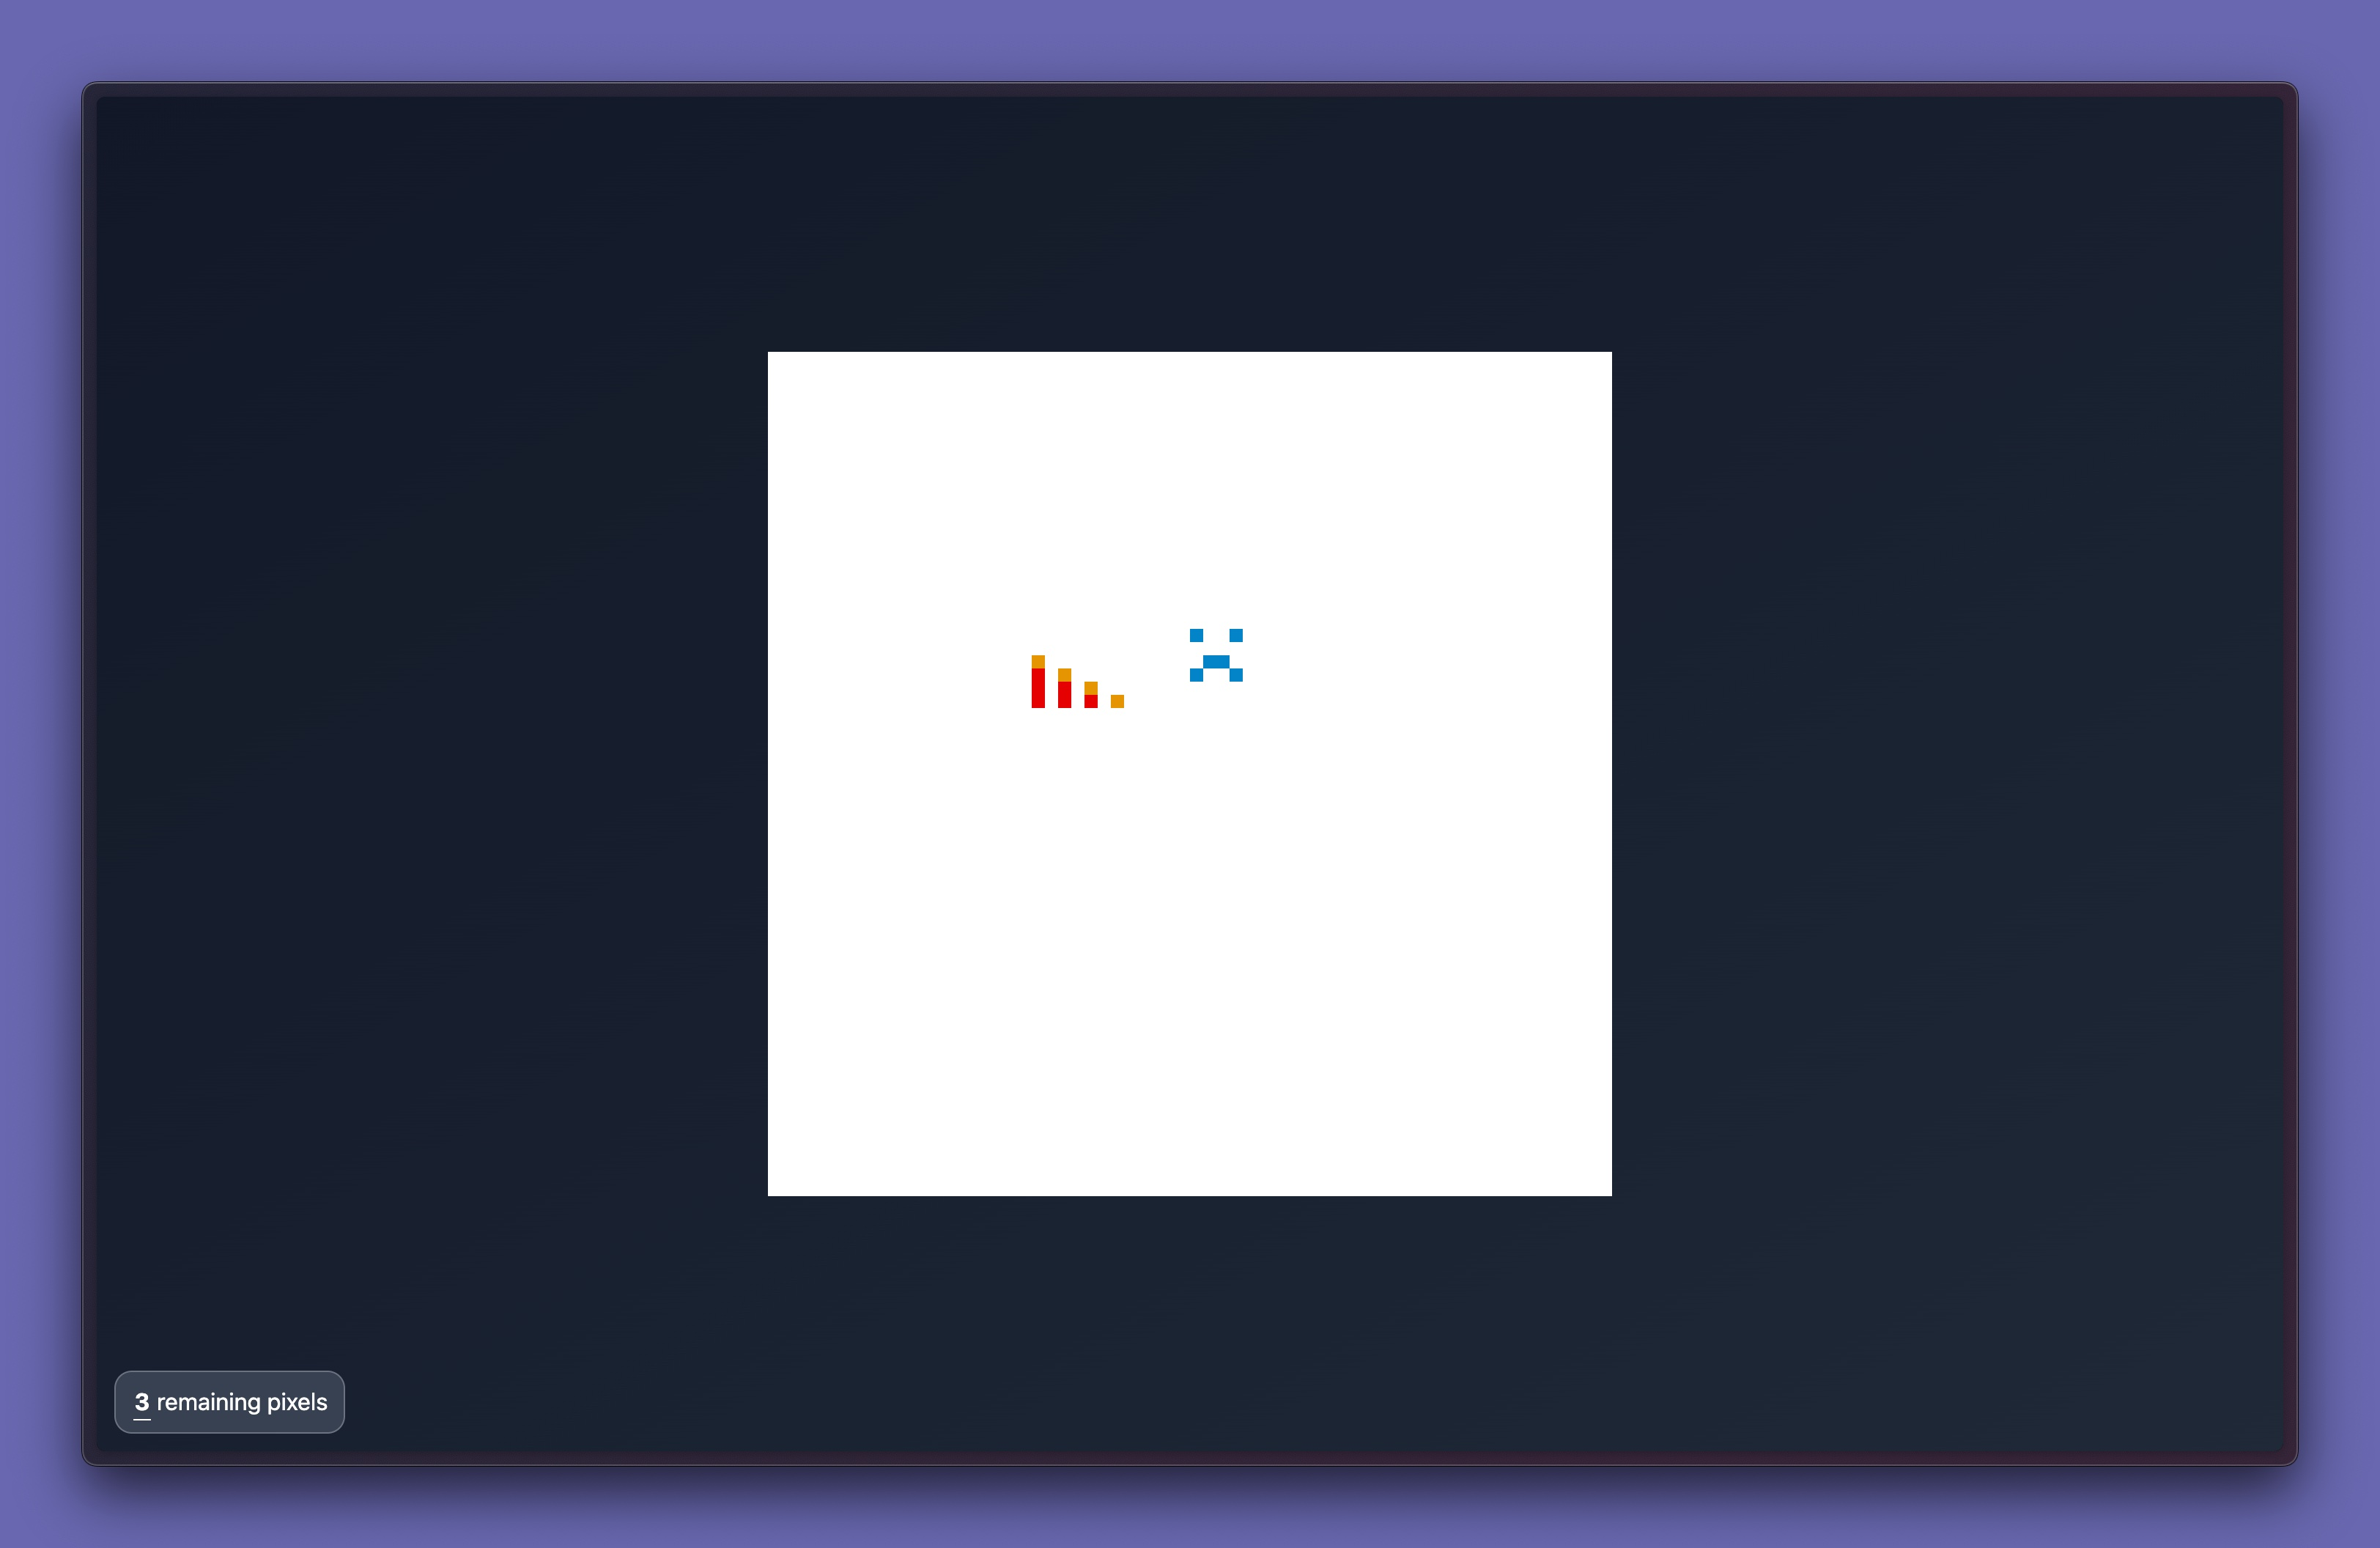
\includegraphics[width=1\textwidth]{./assets/figures/screenshot-app-1.jpeg}
  \caption{Interface de BeePlace sur ordinateur à l'arrivée sur la page}
  \label{fig:screenshot-app-1}
\end{figure}

\begin{figure}[H]
  \centering
  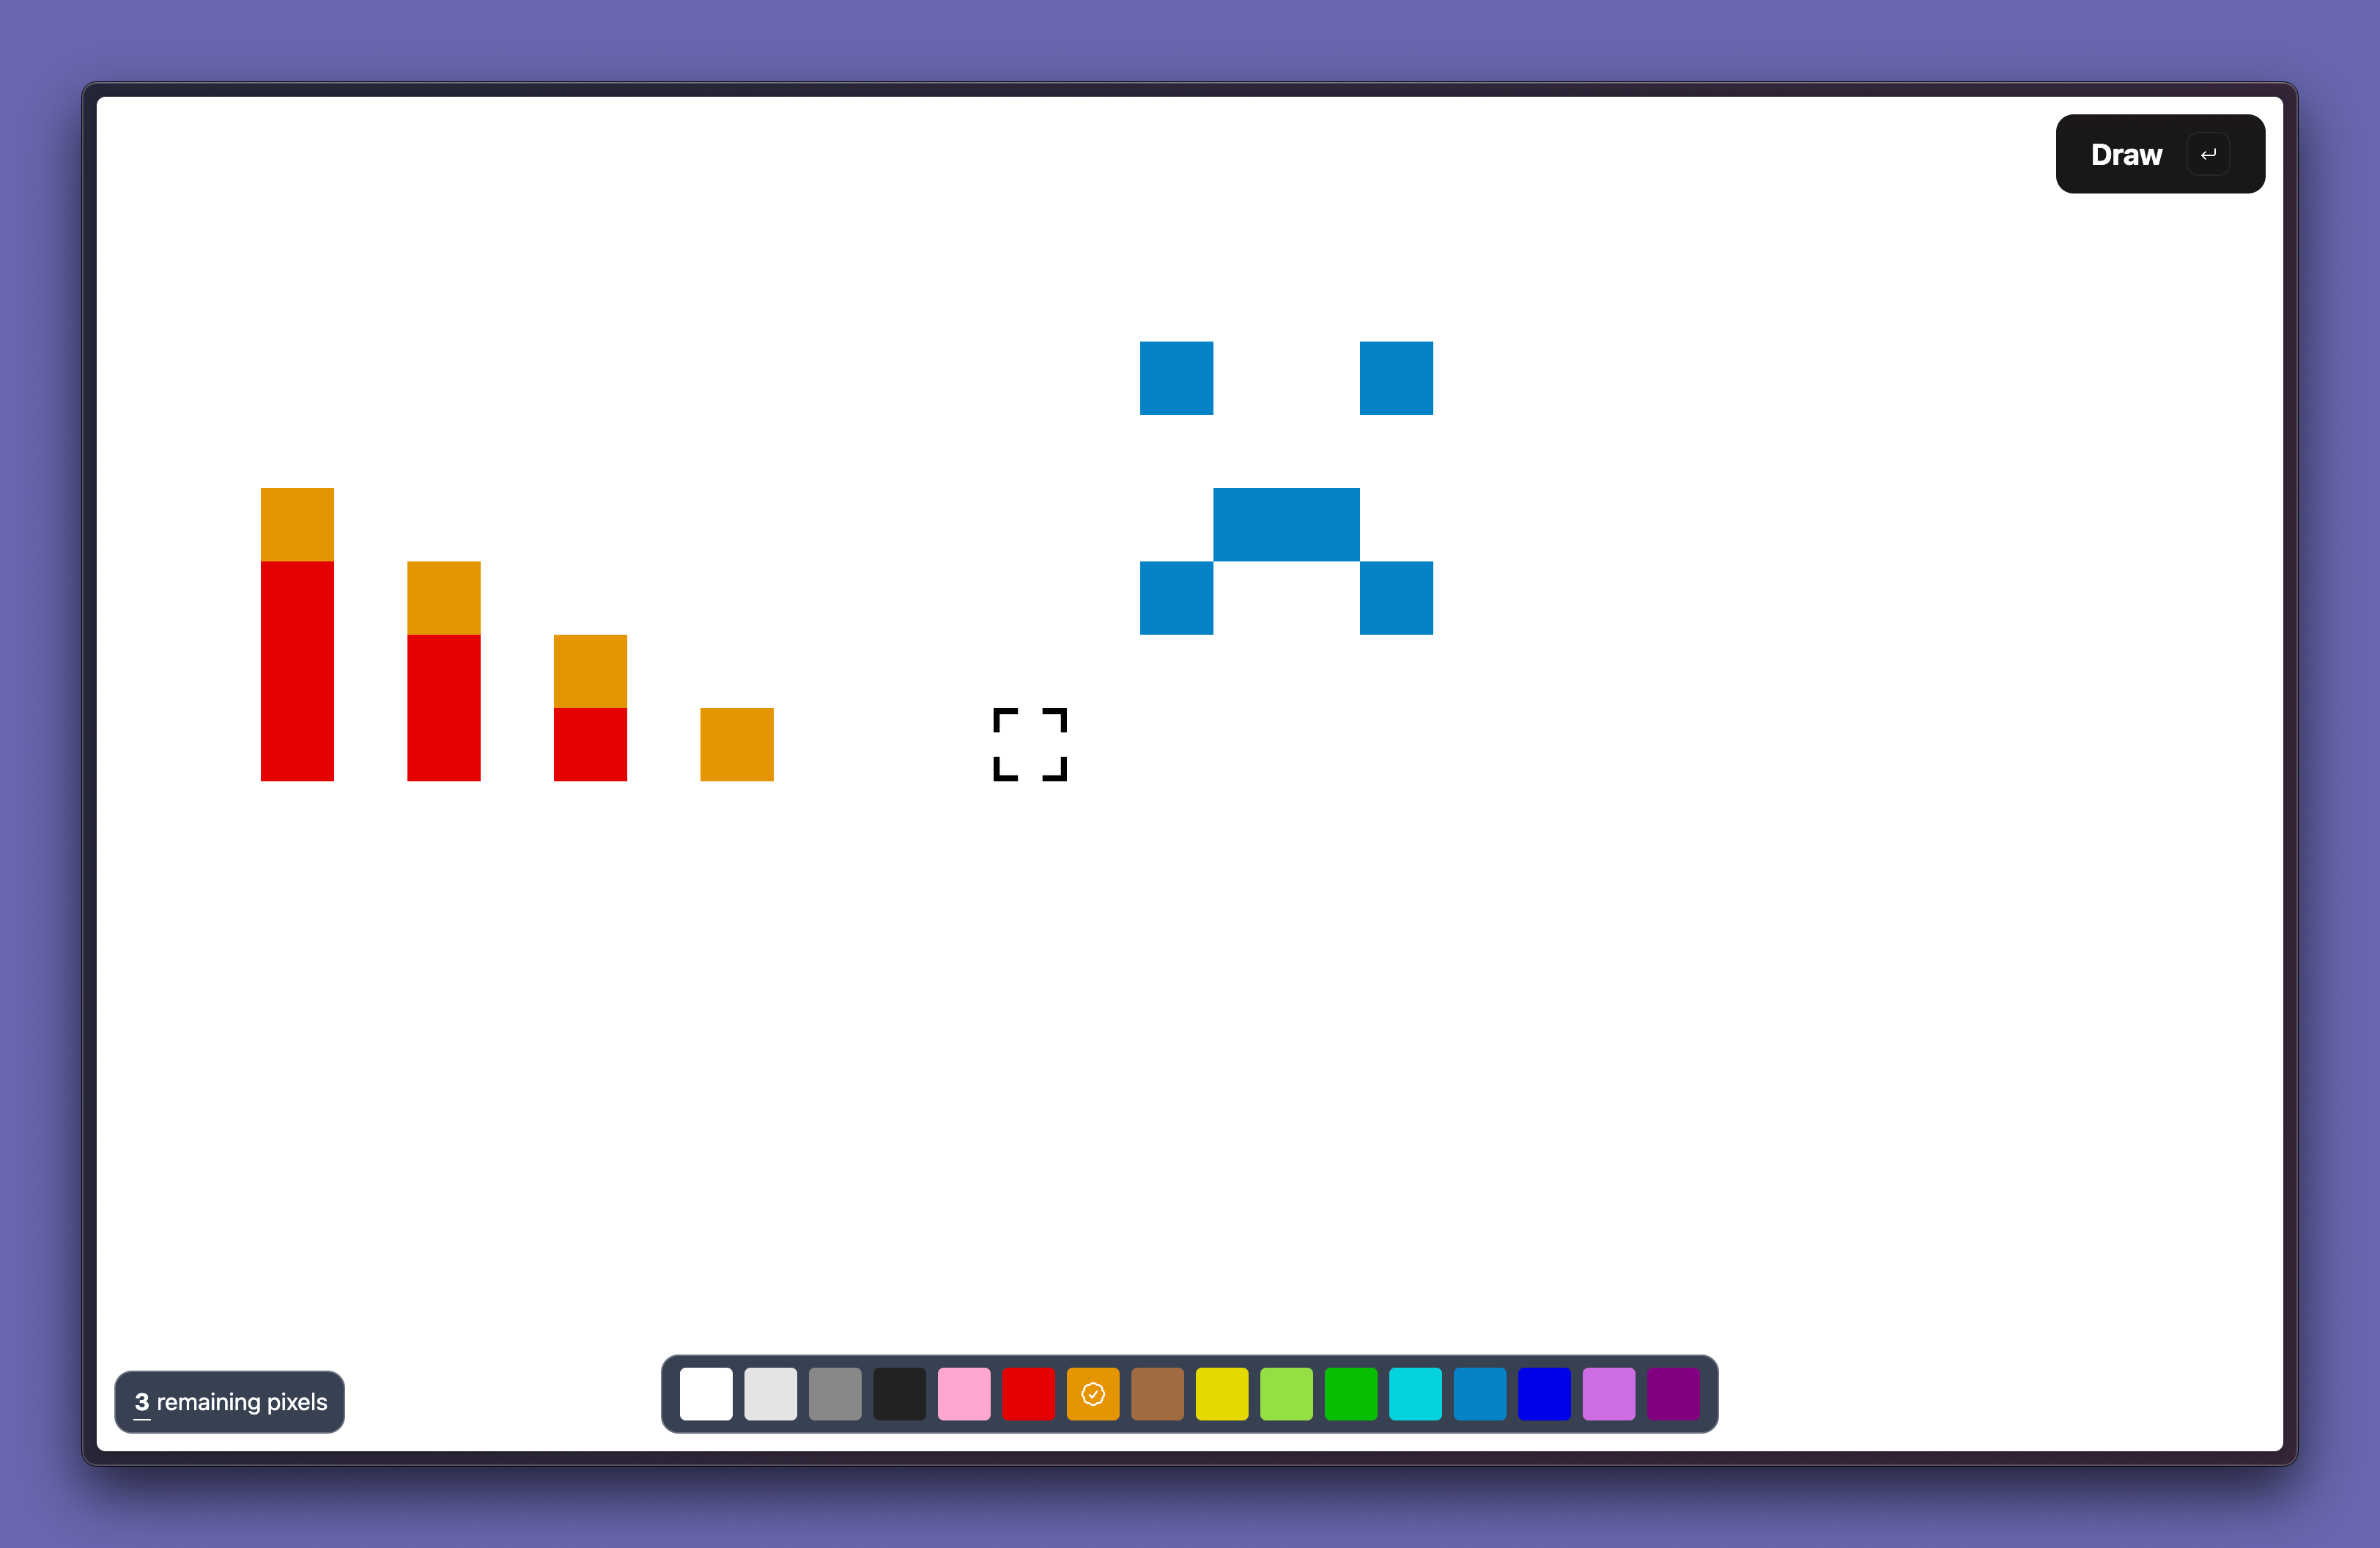
\includegraphics[width=1\textwidth]{./assets/figures/screenshot-app-2.png}
  \caption{Interface de BeePlace sur ordinateur lorsque l'utilisateur clique sur un pixel}
  \label{fig:screenshot-app-2}
\end{figure}

\begin{figure}[H]
  \centering
  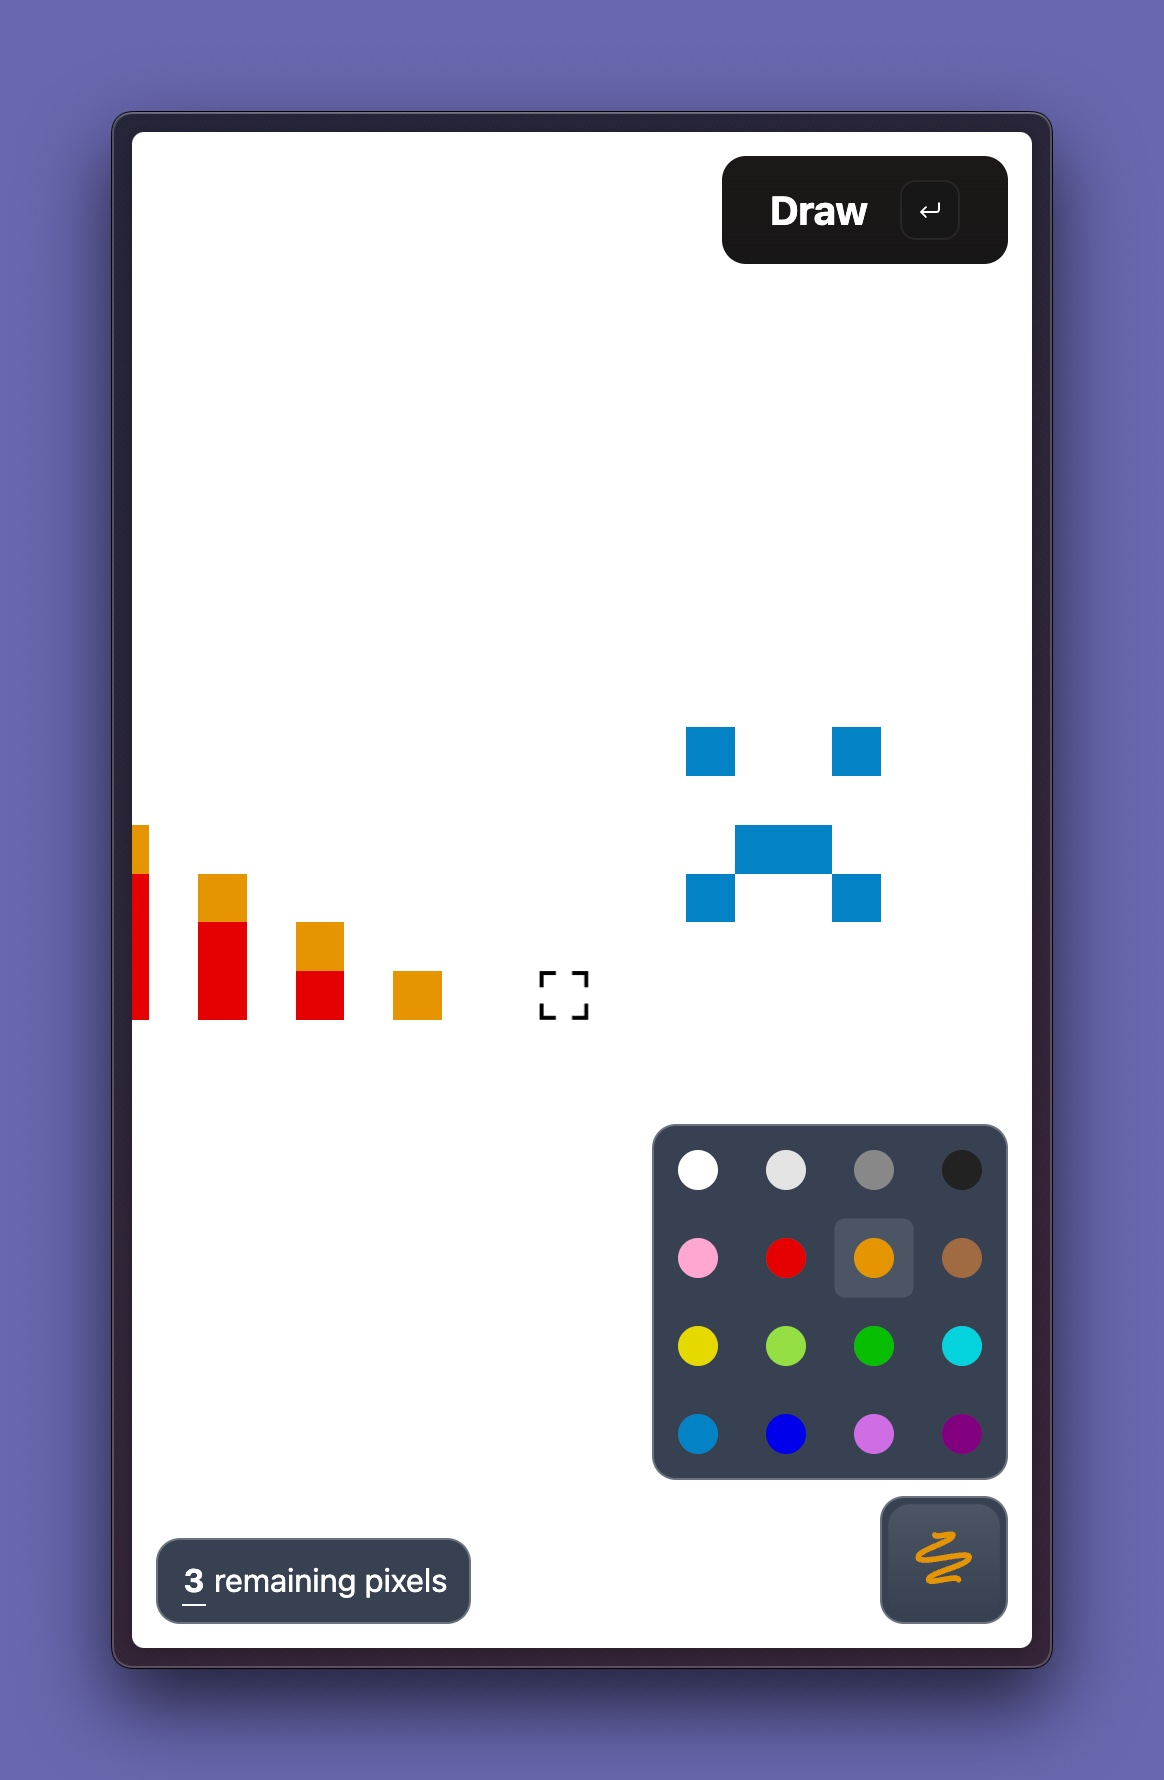
\includegraphics[width=0.5\textwidth]{./assets/figures/screenshot-app-3.jpeg}
  \caption{Interface de BeePlace sur mobile}
  \label{fig:screenshot-app-3}
\end{figure}

\subsection{Canvas}

La toile est le point central de l'application, celle-ci est modélisée grâce à l'élément HTML5 `<canvas>` \cite{canvas}. Cet élément permet de dessiner des formes, des images et du texte. Il est possible de dessiner directement sur le canvas en utilisant le contexte 2D ou 3D. Les formes à dessiner sont très simples dans le cas de \gls{beeplace} car il s'agit de pixels représentés par des carrés de couleurs unies.

\subsubsection{Dessin des pixels}

Deux choix sont possibles pour dessiner les pixels sur le canvas:

\begin{enumerate}
  \item Représenter un pixel comme un pixel du canvas
  \item Représenter un pixel comme un carré de plusieurs pixels du canvas
\end{enumerate}

La deuxième variante permet d'avoir directement une représentation agrandie de la toile. En effet, si la toile a par exemple des dimensions de 64 pixels de largeur, l'utilisateur ne doit pas avoir un canvas de 64 pixels affiché à l'écran, ce qui serait trop petit et illisible. Cependant, représenter un pixel par plusieurs pixels sur le canvas pose problème lorsque l'utilisateur clique sur le canvas pour placer un pixel. En effet, cela demanderait plus de calculs pour connaître les coordonnées réelles du clique de l'utilisateur. La première variante a donc été choisie. Afin de ne pas avoir un canvas trop petit, il est possible de zoomer sur l'élément via la propriété transform en CSS \cite{transformcss}. De base, cela rendrait l'image floue mais il est possible de changer ce comportement en utilisant l'attribut image-rendering \cite{image-renderingcss} avec comme valeur `pixelated`. Comme notre toile est remplie de pixels, cela permet d'avoir un rendu parfaitement net.

\subsection{Pinchzoom}

Écouter les événements utilisateurs pour réaliser des transformations sur un élément (le déplacer, zoomer à un point précis) revient à réaliser ce qu'on appelle un "Pinch-to-Zoom" ou plus simplement "pinchzoom". Ce terme signifie littéralement "pincer pour zoomer". Il s'agit d'un geste utilisé sur les appareils tactiles pour zoomer sur une image ou une page web ainsi que se déplacer. Réaliser une implémentation de ce geste devient vite une tâche fastidieuse. En effet, il est nécessaire d'écouter divers événements différents pour que l'utilisation soit agréable sur tout type d'appareils:

\begin{itemize}
  \item Les événements de la souris
  \item Les événements tactiles
  \item Les événements du pavé tactile qui sont un mélange des deux précédents
\end{itemize}

Adapter le code en fonction de la nature de l'événement devient vite compliqué et source de bug. Heureusement, plusieurs librairies existent afin de faciliter l'implémentation, surtout dans l'écosystème React très riche. La liste qui suit contient les options testées et les raisons pour lesquelles elles ont ou non été retenues.

\subsubsection{React-zoom-pan-pinch}

Le librairie la plus connue se nomme React-zoom-pan-pinch \cite{react-zoom-pan-pinch}. Celle-ci propose un code assez léger, entièrement en \gls{typescript} et sans dépendance externe. Le problème survient lorsque l'utilisateur doit interagir avec l'élément à l'intérieur du Pinchzoom, dans ce cas-ci le canvas. En effet, en plus de pouvoir déplacer et zoomer sur le canvas, l'utilisateur doit pouvoir cliquer sur celui-ci pour placer un pixel. Cependant, la librairie ne permet pas de le faire nativement et un comportement très étrange de translation en dehors de l'écran se produit lors d'un clique. C'est pourquoi cette librairie n'a pas été retenue.

\subsubsection{React-quick-pinch-zoom}

Cette seconde librairie, react-quick-pinch-zoom \cite{react-quick-pinch-zoom} est une adaptation pour React d'une librairie \gls{javascript} plus connue nommée simplement PinchZoom.js \cite{pinchzoomjs}. Le soucis de cette libraire arrive lorsque l'élément à l'intérieur du Pinchzoom doit prendre toute la taille de la fenêtre, ce qui est le cas pour \gls{beeplace}: le canvas est l'élément unique de l'application et prend donc l'intégralité de la page. Lorsque c'est le cas, le comportement de la librairie est étrange et très aléatoire en fonction des événements utilisateurs. Cette seconde librairie n'a donc également pas été retenue.

\subsubsection{React-fast-pinch-zoom}

Heureusement, le même auteur que la seconde librairie a développé une autre version appelée react-fast-pinch-zoom \cite{react-fast-pinch-zoom}. Celle-ci se base cette fois-ci sur une librairie de PinchZoom réalisée par l'équipe de Google Chrome \cite{pinch-zoom-googlechromelabs}. Celle librairie repose elle-même sur une autre libraire de la même équipe Google Chrome, PointerTracker \cite{pointer-tracker}. L'avantage de cette librairie est qu'elle utilise la notion de Pointer events \cite{pointer-events} qui contrairement aux anciens événements, ne partent pas du principe que l'utilisateur utilise une souris. En effet, ces Pointer events sont utilisés pour tous les appareils, que ce soit une souris, un écran tactile ou un pavé tactile.

Malheureusement la librairie, react-fast-pinch-zoom \cite{react-fast-pinch-zoom}, est écrite dans une ancienne manière de faire du React nommée Class component. L'équipe React elle-même recommande d'utiliser des composants en fonction plutôt que des classes "We recommend defining components as functions instead of classes." \cite{react-class-component}. C'est pour cette raison que le code de la librairie a été copié dans le projet et adapté pour être utilisé avec des composants en fonction.

\subsection{Gestion du state}

L'application React doit garder un état à jour. Cet état comporte plusieurs éléments:

\begin{itemize}
  \item Les réglages initiaux de la toile comme sa taille, les couleurs disponibles, le temps d'attente entre chaque pixel, etc.
  \item Le nombre de pixels posés par l'utilisateur dans l'intervalle de temps.
  \item Le moment où l'utilisateur pourra à nouveau placer un pixel.
\end{itemize}

Toutes ces variables sont utilisées dans de nombreux composants React. Il est donc nécessaire de les stocker dans un endroit centralisé afin de pouvoir les utiliser facilement sans devoir les faire passer sur plusieurs niveaux d'imbrication. Pour cela, il existe principalement deux solutions:

\begin{enumerate}
  \item Utiliser une librairie externe de stockage de state.
  \item Utiliser le state fourni par React dans un Contexte \cite{react-context} afin de le rendre accessible à tous les composants enfants.
\end{enumerate}

\subsubsection{Librairie externes}

De nombreuses librairies existent pour gérer le state d'une application React. La plus connue est Redux \cite{react-redux}. Cependant, Redux est une librairie assez lourde et complexe à mettre en place. Elle est également très verbeuse. Il existe des alternatives plus légères et simples comme Zustand \cite{zustand}.

Les avantages de Zustand sur Redux sont les suivants:
\begin{itemize}
  \item Plus simple et sans opinion donc plus facile à prendre en main.
  \item Zustand utilise les hooks de React comme moyen principal de consommer le state, sa syntaxe est donc plus proche de React.
  \item Zustand peut modifier le state sans forcer le composant à se re-rendre, ce qui peut être utile au niveau des performances.
\end{itemize}

\subsubsection{Contexte React}

Au lieu d'installer une libraire externe, il est possible d'utiliser le Contexte React \cite{react-context}. Celui-ci permet de stocker des données ainsi que des fonctions utilitaires dans un endroit centralisé et de les rendre accessibles à tous les composants enfants. Cependant, les contextes amènent plusieurs problèmes:

\begin{itemize}
  \item Un contexte React n'est pas fait pour stocker des données qui changent souvent. En effet, à chaque changement de state, tous les composants enfants sont re-rendus, ce qui peut être problématique au niveau des performances.
  \item Créer un contexte est assez verbeux et nécessite beaucoup de code pour un résultat assez simple.
  \item Le state dans un contexte n'est pas toujours accessible et à jour. Dans des fonctions de callback d'événements par exemple ou d'événements WebSockets, il faut utiliser des astuces afin de pouvoir accéder au state.
\end{itemize}

C'est pourquoi il est préférable d'utiliser une librairie externe comme Zustand.

\section{Backend}

\subsection{Identification des utilisateurs}
La bonne identification des utilisateurs est un point crucial de l'application. En effet, il est nécessaire de pouvoir vérifier que les utilisateurs attendent bien le temps nécessaire avant de pouvoir placer un nouveau pixel. Pouvoir contourner cette règle casserait complètement le but principal de l'application qui est de faire collaborer les utilisateurs.

Ajouter une authentification classique avec un pseudonyme et un mot de passe ou même via un réseau social n'est pas envisageable. En effet, cela ajouterait trop d'étapes à l'utilisateur avant de pouvoir placer un pixel. L'application a pour but d'être utilisée dans des milieux festifs, il faut donc que les usagers aient le moins de barrière possible pour pouvoir l'utiliser.

Identifier les utilisateurs sans véritable authentification n'est pas trivial. L'idée est d'utiliser les empreintes digitales des joueurs, plus souvent appelées fingerprint \cite{devicefingerprint}. Cela a pour but d'empêcher aux utilisateurs de contourner la règle du temps d'attente en rafraîchissant la page, en utilisant une navigation privée ou en changeant de navigateur.

\subsubsection{Fingerprint}

Cette technique consiste à récupérer des informations sur le navigateur de l'utilisateur afin de créer un identifiant unique, notamment via les caractéristiques techniques de l'appareil comme sa résolution d'écran ou ses polices installées. La liste des attributs utilisés se doit d'être la plus grande possible afin d'éviter au maximum les collisions entre les utilisateurs. Un exemple plus détaillé sera présenté dans la prochaine sous-section. De plus, les informations doivent être stables afin que l'identifiant de l'utilisateur ne change pas. A partir de toutes ces caractéristiques, l'identifiant est créé via une fonction de hachage.

Ces méthodes demandent des algorithmes complexes et il est donc préférable d'utiliser une librairie existante. Malheureusement, le choix est limité. La librairie FingerprintJS \cite{fingerprintjs} est la plus populaire mais possède une version propriétaire payante. L'idée de ce travail de Bachelor n'est pas de dépendre de multiples services tiers, que ce soit pour le déploiement ou pour le développement. C'est cette raison qui a poussé à chercher d'autres possibilités.

La seule vraie alternative open source se nomme Broprint.js \cite{broprintjs}. Malheureusement, après quelques tests sur un échantillon de quelques personnes, des collisions d'identifiants ont déjà eu lieu car les ordinateurs potables étaient du même modèle. De plus certains utilisateurs avaient un identifiant différent à chaque chargement de la page, ce qui n'est pas acceptable.

% , comme annoncé lors de la réalisation du POC \ref{poc-ameliorations},

\subsubsection{FingerprintJS}
Le choix se tourne donc finalement vers FingerprintJS \cite{fingerprintjs}. Il existe deux versions de la librairie, une gratuite et open source et la deuxième déjà mentionnée propriétaire. Ce qui permet de garder un code sans service tiers en utilisant la version open source. FingerprintJs annonce entre 40\% et 60\% de précision pour la version gratuite contrairement à la version payante qui tourne aux alentours de 99.5\% \cite{fingerprintjsrepo}. Cette différence est due principalement au fait que la version gratuite contient uniquement du code exécuté côté client, sur le navigateur de l'utilisateur.

Afin d'avoir une idée des caractéristiques utilisées par FingerprintJS, \href{https://fingerprintjs.github.io/fingerprintjs}{un exemple de résultat} est donné sur leur site. La liste est conséquente, elle contient notamment:

\begin{itemize}
  \item Les polices installées, leurs préférences
  \item Les réglages du navigateur comme sa langue, ses fonctionnalités activées ou pas etc.
  \item Les réglages de l'ordinateur comme le son, les couleurs, etc.
  \item Les informations sur la machine physique comme la résolution d'écran, le nombre de coeurs, la mémoire vive, etc.
\end{itemize}

En plus de toutes ces caractérisées, FingerprintJS utilise la notion de Canvas Fingerprint qui consiste à dessiner une image sur un canvas HTML5 (non affiché à l'utilisateur) et de récupérer le résultat sous forme de chaîne de caractères. Des variables comme le temps de rendu graphique sont utilisées afin de différencier chaque utilisateur.

Pour finir, l'avantage supplémentaire de FingerprintJS est que la version payante dispose d'un essai gratuit d'un mois et que la migration entre les deux versions contient littéralement deux lignes \cite{migratefingerprintjs}. Il suffit de changer le nom du package installé et d'ajouté la clé à notre compte FingerprintJS pour basculer sur la version payante. Il est donc envisageable d'utiliser la version gratuite en règle générale et de basculer sur la version payante lors des événements importants, comme le Baleinev festival.

\subsection{Configuration}

Pour pouvoir modifier facilement la configuration de la toile, celle-ci est configurée grâce à des variables d'environnement du côté du Backend. En effet, le backend transmet toutes ces valeurs au frontend lors de la première connexion comme expliqué dans la prochaine section \ref{section:connexion-websockets}. Les variables d'environnement intéressantes sont présentées dans le listing \ref{listing:env-variables}.

\begin{listing}[H]
  \begin{minted}{bash}
# The width and height of the board
BOARD_SIZE=64

# The time in seconds user need to wait before they can place another pixel
COOLDOWN=10

# Array of colors in hex format
COLORS='["#FFFFFF","#E4E4E4","#888888","#222222","#FFA7D1","#E50000","#E59500", ...]'

# The default stroke color id
INITIAL_COLOR=3

# The default zoom level
INITIAL_SCALE=9

# The number of pixels a user can place before they need to wait
MAX_PIXELS=3
\end{minted}
  \caption{Variables d'environnement de configuration de la toile}
  \label{listing:env-variables}
\end{listing}

En plus des variables présentées, d'autres plus classiques sont utilisées pour la connexion avec Redis ou choisir le port sur lequel tourne l'application par exemple.

\subsubsection{Validation des variables d'environnement}

Les variables par défaut sont définies dans un fichier \texttt{.env.defaults} qui sera copié dans un fichier \texttt{.env} lors de l'installation du projet. Ce fichier \texttt{.env} est utilisé et chargé par le backend et n'est pas versionné sur le répertoire git. En plus de ces deux fichiers, un troisième est défini appelé \texttt{.env.schema}. Ce fichier contient la liste des variables d'environnement ainsi que leur structure sous la forme d'une Regex. Ce fichier est utilisé par le package \texttt{dotenv-extended} \cite{dotenv-extended} qui permet de valider les variables d'environnement. Si une variable d'environnement est manquante ou si sa valeur ne correspond pas à la Regex définie dans le fichier \texttt{.env.schema}, le backend ne démarre pas et affiche un message d'erreur. Ces tests sont également effectués dans la pipeline de CI/CD afin d'éviter les erreurs inutiles.

\subsection{Connexion WebSockets}
\label{section:connexion-websockets}

\fig[H, width=0.8\textwidth]{Diagramme de séquence de la connexion WebSockets}{sequence-websockets.svg}

Comme démontré dans la figure \ref{sequence-websockets.svg}, le Backend envoie l'état actuel de la toile ainsi que les diverses variables d'environnement servant à la configuration lorsque la connexion WebSockets est initiée par le client.

Lorsque le client reçoit cet événement \texttt{INIT\_BOARD}, il envoie à son tour un événement \texttt{FINGERPRINT} au Backend qui contient son empreinte numérique. Le Backend stocke ensuite cet identifiant dans le Socket utilisé pour la connexion avec ce client pour que le client n'ait pas besoin de l'envoyer à chaque nouvelle requête.

Après cette première connexion, le client peut envoyer des événements pour poser des pixels et le serveur envoie lui des événements pour notifier le client de changements sur la toile réalisés par d'autres utilisateurs.

\subsection{Stockage de l'état actuel de la toile}
\label{section:stockage}

Redis offre de nombreuses manières de stocker des données. La première option est de stocker chaque couleur de pixel dans une clé en utilisant les coordonnées (x, y) comme clé. Cependant, récupérer un nombre important de clés en une fois (lors du chargement initial de la toile) n'est pas efficace. En effet, il faut scanner les différentes clés en spécifiant un paterne à trouver. Il est donc préférable de stocker l'état de la toile dans une seule clé Redis. Pour cela, il est possible d'utiliser le type de données Bitfield \cite{bitfield} de Redis. Ce type de données permet de stocker des bits dans une clé Redis et toutes les opérations se font en \bigO{1}. Il s'agit de la structure de données utilisée par l'équipe de \gls{reddit} dans leurs applications r/place de 2017 et 2022. Le Senior Software Engineer de Daniel Ellis a notamment donnée une conférence expliquant leur utilisation de Redis lors de la RedisConf 17 \cite{redisconf}. L'implémentation qui suit est donc basée sur les informations données dans cette conférence.

Afin de convertir la toile en une suite de bits, il est nécessaire de donner un id à chaque couleur afin de ne pas stocker un nombre incalculable de chaîne de caractères correspondant aux différentes couleurs. Pour avoir une marge concernant le nombre de couleurs disponibles, le type de chaque élément du Bitfield a été spécifié comme un entier non signé sur 8 bits. Cela permet de stocker 256 couleurs à la place des maximum 16 disponibles avec 4 bits. Le second avantage à utiliser 8 bits et qu'il rend possible l'utilisation d'un Uint8ClampedArray \cite{uint8clampedarray} du côté du client afin de créer une image du contenu du canvas très simplement sans avoir à faire de conversion.

Pour calculer l'offset du bit à modifier en fonction de la position du pixel (x, y), il est possible d'utiliser la simple formule suivante:
\begin{equation}
  offset = (y * width + x)
\end{equation}

Pour avoir accès l'entièreté du canvas, il suffit de récupérer la clé Redis sans préciser d'offset. Il est ainsi possible d'avoir accès à un tableau d'entiers représentant les couleurs de chaque pixel de la toile.

\subsection{Stockage de l'historique}

Comme précisé précédemment, le Bitfield Redis n'a aucune idée des états passés de chaque pixel. De plus, il ne contient aucune information concernant la date ou l'utilisateur ayant posé le pixel. La conception de ces données a été réalisée dans une table unique nommée \texttt{pixel} contenant les champs suivants:

\begin{itemize}
  \item id: Identifiant unique de l'historique
  \item x: Position x du pixel
  \item y: Position y du pixel
  \item color: Identifiant de la couleur du pixel
  \item created\_at: Date et heure à laquelle le pixel a été posé
  \item user: Identifiant de l'utilisateur ayant posé le pixel
\end{itemize}

\subsection{Gestion de la durée d'attente entre la pose de pixels}

Redis est également utilisé pour vérifier que le temps d'attente entre chaque pixel est bien respecté pour chaque utilisateur. En effet, il est possible de stocker des données dans Redis avec une durée de vie, qui correspond ici au temps d'attente.

Chaque utilisateur est stocké selon le format de clé suivant: \mintinline[breaklines]{bash}{users:<fingerprint>}. La clé aurait simplement pu être la fingerprint de l'utilisateur mais la préfixer avec \texttt{users:} permet de pouvoir sélectionner rapidement toutes les clés des utilisateurs via un scan. Cela peut être utile pour la remise à zéro des temps d'attente par exemple. Concernant la valeur associée à la clé, il s'agit simplement du nombre de pixels posés par l'utilisateur durant l'intervalle. S'il s'agit du premier pixel, la clé est créée et le temps d'attente démarre. Pour les pixels suivants, la valeur est incrémentée grâce aux méthodes que Redis nous offre. Si le nombre de pixels stockés est égal au nombre maximal de pixels autorisés, l'opération est simplement refusée.

\subsection{Administration}

Pour protéger les actions réalisables uniquement par des administrateurs, une authentification doit être mise en place. L'implémentation se base sur le module Passport \cite{passport} qui est le standard en matière d'authentification dans le monde \gls{nodejs}. Passport propose des centaines de manières de s'authentifier, appelées stratégies. Celle choisie se nomme HeaderAPIKey \cite{passport-headerapikey} et permet de vérifier qu'une clé d'API est présente dans les entêtes de la requête HTTP. Cette clé est ensuite comparée à la valeur stockée comme variable d'environnement \mintinline[breaklines]{bash}{API_KEY}. Si la clé est correcte, l'utilisateur est considéré comme authentifié et peut effectuer les actions réservées aux administrateurs.

\subsubsection{Remise à zéro de la toile}

Voici un exemple d'appels HTTP en ligne de commande sur la route permettant de remettre à zéro la toile pour tous les utilisateurs. Lorsque la clé d'API est incorrecte ou absente, une erreur 401 est retournée nous signifiant que l'utilisateur n'est pas autorisé à effectuer cette action.

\begin{minted}[breaklines]{bash}
  # Version sans clé dans l'entête ou clé incorrecte
  curl http://localhost:4000/board
  {"statusCode":401,"message":"Unauthorized"}%

  # Version avec clé correcte dans l'entête
  curl http://localhost:4000/board --header "apiKey: API_KEY"
  {"status":"ok","message":"Board reset"}%
\end{minted}

Grâce à l'implémentation de l'authentification sous la forme d'un décorateur \gls{typescript} \cite{typescript-decorators}, il est possible de protéger simplement les méthodes souhaitées. En effet, les décorateurs permettent d'ajouter des fonctionnalités à une méthode sans avoir à la modifier, en s'injectant directement dans le contexte de celle-ci. Par exemple, la méthode permettant de remettre à zéro la toile est protégée par le décorateur \texttt{ApiKeyAuth}:

\begin{minted}[breaklines]{typescript}
@Get()
@ApiKeyAuth()
async reset() {
  await this.boardGateway.resetBoard();

  return {
    status: 'ok',
    message: 'Board reset',
  };
}
\end{minted}

La méthode \texttt{resetBoard} du BoardGateway supprime simplement la clé Redis contenant l'état complet de la toile. De plus, tous les utilisateurs connectés sur l'application sont notifiés de la remise à zéro de la toile grâce à un événement WebSockets et leur canvas est vidé. Cela permet de ne pas avoir à recharger la page pour voir la toile se vider. Ce qui n'aurait pas été pratique car le but principal de cette fonctionnalité et de censurer rapidement les oeuvres inappropriées.
